\chapter{Visualisierungen} \label{ch:Visualisierung}

Diverse Daten - beispielsweise Simulationsergebnisse - erfordern eine geeignete Aufbereitung und ansprechende Darstellung. In diesen Darstellungen können Zusammenhänge zwischen verschiedenen abhängigen Größen gezeigt werden, oder mit anderen verglichen werden.
Bei dynamischen Systemen sind oft die Zeitverläufe der Systemgrößen von Interesse, die für Analysen in Diagrammen gezeigt werden können. Für einen Überblick über das Verhalten eines Systems bieten sich darüber hinaus Animationen an.

In dem folgenden Abschnitt werden einige Erläuterungen zu der Animation der mobilen Betonpumpe gegeben. Bei sämtlichen abgebildeten Diagrammen stehen alle notwendigen Anmerkungen an den entsprechenden Stellen, so dass hier nicht weiter darauf eingegangen wird.

\section{Animation}

\begin{figure}[h]
\centering
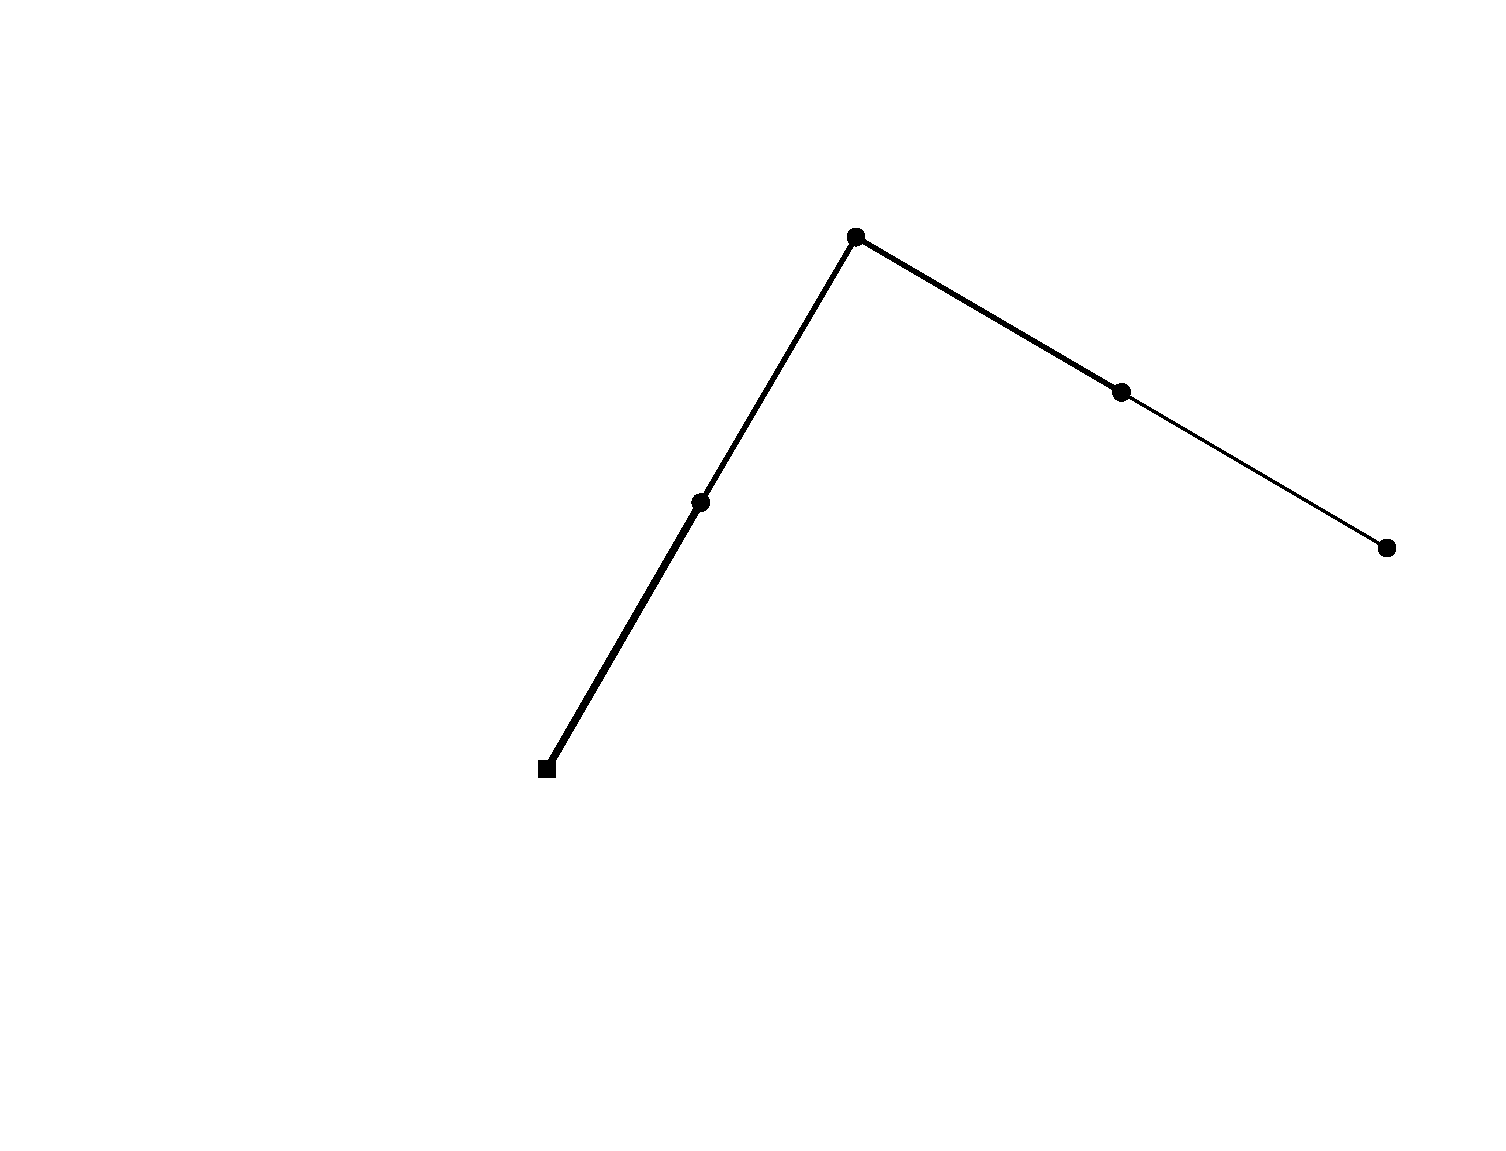
\includegraphics[width=0.7\linewidth]{animation01}
\caption[Animation Betonpumpe]{Animationsgrafik von 2 Gliedern (Auslegern) einer mobilen Betonpumpe}
\label{fig:animation}
\end{figure}

In der Abbildung \ref{fig:animation} sind zwei Glieder einer mobilen Betonpumpe mit zwei Auslegern abgebildet. Beide Träger wurden in der Modellbildung durch ein elastisches Knickgelenk in ihrer Mitte den realen Gegebenheiten angenähert. An dieser Stelle treten die unerwünschten Effekte auf, die es im Laufe des Seminars zu verringern gilt. 